\section{Gradient-based learning}

\mode<presentation>{
\begin{frame}{Where are we?}

\begin{columns}
    \begin{column}{0.55\textwidth}
        \tableofcontents[currentsection,hideallsubsections]
    \end{column}
    \vrule{}
    \begin{column}{0.45\textwidth}
        \begin{center}
            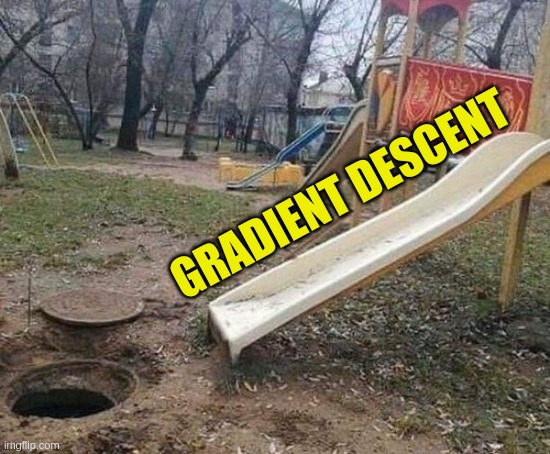
\includegraphics[width=0.85\textwidth]{img/meme_slide}
        \end{center}
        \begin{center}
        Iterative, step-by-step\\
        minimization\\
        of the training error.
        \end{center}
    \end{column}
\end{columns}
\end{frame}
}

\begin{frame}\frametitle{Minimizing the training error}
	Training error $E^T$ for the training set $\left\{(\vec x^{(\alpha)}, y^{(\alpha)}_{T})\right\}$: 
    \begin{equation}
        \ETw = \frac{1}{p} \sum\limits_{\alpha = 1}^p 
					e\tyxwalpha
    \end{equation}
    
    \mode<article>{
    The objective is to minimize the training error w.r.t. the model parameters $\vec w$. That is
    }
    
    \begin{equation}
        \ETw \eqexcl \min_{\vec w} \quad \Rightarrow \quad \vec w^{*} = \argmin_{\vec w} \ETw
    \end{equation}

    \begin{figure}[h]
        \centering
        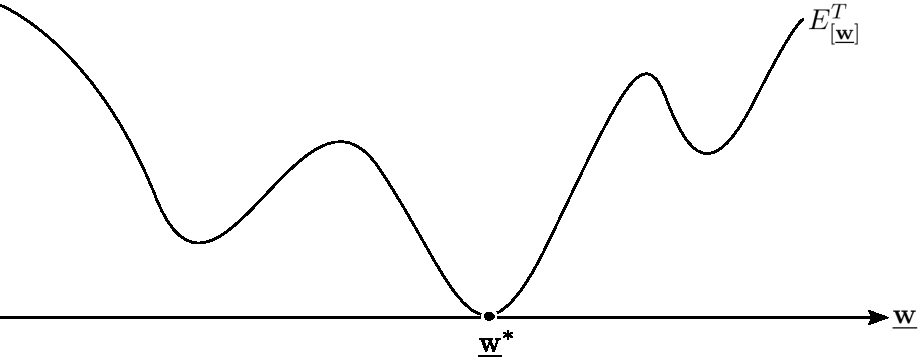
\includegraphics[height=2.5cm]{img/section1_fig19_no_steps}
        \caption{Training error with minimum at $\vec w^{*}$}
        \label{fig:training_error} 
    \end{figure}
    \slidesonly{\vspace{-10mm}}
    
    \pause 
    \question{What is the strategy for finding $\vec w^{*}$ analytically?}

\end{frame}

\subsection{Finding the minimum of the training error analytically}

\begin{frame}\frametitle{\subsecname}

    Example with a simple connectionist neuron model
    with parameters
    $$\vec w = (w_{0}, w_{1}, \ldots, w_{N})^{\top}$$

    The strategy for finding the minimum of a function $\ETw$ analytically\notesonly{ is as follows}:
    %\pause
    \begin{enumerate}
    \item<1-> Compute the gradient w.r.t. $\vec w$ by taking the first partial derivatives w.r.t to each component in the vector $\vec w$
    \begin{equation}
        \frac{\partial \ETw}{\partial \vec w} = \left(\,
        \frac{\partial \ETw}{\partial w_{0}}, \,
        \frac{\partial \ETw}{\partial w_{1}}, \,\ldots\,,\, 
        \frac{\partial \ETw}{\partial w_{N}}\,
        \right)^{\top}
        \label{eq:gradient_partial}
    \end{equation}
    \only<1>{The gradient $\frac{\partial \ETw}{\partial \vec w}$ has the same dimensionality as $\vec w$.}
    
    \item<2-> Set the gradient to zero: $\frac{\partial \ETw}{\partial \vec w} \eqexcl \vec 0$
    \item<3-> Solve for $\vec w$ to find extrema.
    \item<4-> Select solution corresponding to global minimum.
    
    \end{enumerate}
    \only<5->{
        Caveat: Closed-form solution infeasible for complex models such as MLPs.
        \mode<presentation>{
        Instead: Iterative learning algorithm gradient descent.
        }
    }
\end{frame}


